\documentclass{article}

\usepackage{iclr2026_conference,times}
\usepackage{hyperref}
\usepackage{url}
\usepackage{booktabs}
\usepackage{amsmath}
\usepackage{amssymb}
\usepackage{amsthm}
\usepackage{graphicx}
\usepackage{array}

\input{math_commands.tex}

\newtheorem{lemma}{Lemma}
\newtheorem{proposition}{Proposition}
\newtheorem{definition}{Definition}

\title{Embodied World Model Repair Loops}

\author{Anonymous Authors\\
Paper under double-blind review}

\begin{document}

\maketitle

\begin{abstract}
Robot world models are often trained, adapted, or selected by prediction quality: next-state error, rollout likelihood, uncertainty, latent reconstruction, or global system-identification fit. For embodied planning, this objective can miss a sharper failure mode. A planner is not an average-case evaluator of a model; it actively searches for useful transitions. A rare false affordance can therefore dominate behavior while contributing almost nothing to global prediction error. This paper studies \emph{Counterexample-Conditioned Repair Automata} (CCRA), a planner-facing wrapper that turns execution contradictions into guarded transition patches used immediately by the next planning call. The claim is intentionally modest. Exact CCRA in a deterministic exact-guard grid is equivalent to one-mismatch transition blocking; the contribution is the repair contract, its scope, and its evaluation target rather than a complicated new learner. We support the claim with a RAM-light full-scale simulation pass: 34,880 streamed per-episode evaluations across critical sparse faults, off-route prediction noise, threshold delay, guard scope, nonstationary stale patches, stochastic contradictions, and planner-exploitation stress. In the largest stress suite, nominal and shield-only models have low final prediction error (0.003) but zero success and 252.3 first-episode counterexamples. Exact CCRA and cost-based avoidance reach 1.00 success after 1.0 first-episode counterexample; threshold-8 repair reaches 1.00 success but pays 8.0 first-episode counterexamples; row guards also solve but raise control-weighted prediction error from 0.028 to 0.264 with a 0.87 false-block rate. The evidence supports a narrow mechanism-level thesis: for embodied agents, the update object should sometimes be the planner-facing transition contract, not global predictive fidelity alone.
\end{abstract}

\section{Introduction}

World models give a robot an internal contract between state, action, and physical consequence. The contract may be a learned dynamics model, a visual prediction model, a latent imagination model, a simulator parameterization, a symbolic transition model, or a language-conditioned affordance map. Modern model-based robot learning and planning have made this contract increasingly useful: learned dynamics can drive model predictive control \citep{lenz2015deepmpc,nagabandi2018neural,chua2018pets}; latent models can support imagination and control \citep{ha2018worldmodels,hafner2019planet,hafner2020dreamer}; visual foresight can optimize action sequences from predicted pixels \citep{ebert2018visual}; online adaptation and system identification can update dynamics under deployment shift \citep{fu2016oneshot,yu2017uposi}; and sim-to-real methods try to make policies and models survive distribution change \citep{tobin2017domain,tan2018sim,jeong2020self}.

This paper does not dispute that prediction quality matters. It asks when prediction quality is the wrong center of the update. The reason is simple: a robot planner is an optimizer. It searches for low-cost or high-value trajectories under the model it has. If one rare transition falsely says that a push clears an object, a wheel crosses a patch, a gripper avoids a catch, or a tool slides through a gap, the planner will preferentially exploit that transition. The error may be a negligible fraction of the transition table, a tiny term in a next-frame loss, or a low-probability event under a passive dataset. Yet it can fully determine behavior.

The update needed after such a failure is not necessarily a globally better model before the next action. It may be much smaller and more urgent: stop authorizing the false transition that execution just contradicted. If a planned action in state $s$ was rolled out as successor $\hat{s}'$ and execution observed $s^\star\neq \hat{s}'$, the next planner call should not be allowed to rely on the same modeled effect as though nothing happened. This is the repair obligation studied here.

We call the mechanism \emph{Counterexample-Conditioned Repair Automata} (CCRA). A CCRA wraps a nominal world model with an ordered set of guarded patches. Each patch stores a guard over state-action contexts, a replacement or forbidden-affordance transition, support metadata, and a planner-facing obligation. Planning rolls out the patched transition relation. Execution contradictions add or strengthen patches. A later learner may consolidate patches into a neural model, simulator parameter, symbolic predicate, or residual dynamics module, but the immediate control loop does not wait for that consolidation.

The contribution is deliberately narrow. Online adaptation, residual learning, uncertainty-aware MPC, shields, active data collection, and model reconciliation are all serious hostile prior work. Exact CCRA is not algorithmically deep in deterministic finite systems; it collapses to one-mismatch transition blocking. The point is to make the planner-facing repair object explicit, to define the failure metrics that expose prediction-success decoupling, and to measure the scope and stale-memory tradeoffs that determine whether repair helps or harms.

The paper makes four contributions.
\begin{enumerate}
    \item It defines CCRA as a planner-facing repair wrapper for embodied world models.
    \item It states narrow formal facts: exact repair prevents repeated exploitation of the same deterministic transition, and thresholded repair pays a predictable counterexample delay.
    \item It reports a full-scale local simulation pass with 34,880 streamed per-episode evaluations, seven stress suites, and stronger baselines than the original short paper.
    \item It gives a claim audit: the evidence supports planner-facing transition repair as a mechanism-level update target, but does not establish hardware performance, learned guard formation, 3D contact generality, or superiority over exact signed/known mechanics.
\end{enumerate}

\section{Motivating Failure Mode}

Consider a robot with a nominal model $T_0$ and a planner that searches paths under $T_0$. The planner repeatedly chooses an action because $T_0$ says it will advance the task. Execution then returns the same state because contact sticks, an object jams, a wheel slips, or an obstacle catches. If $T_0$ is unchanged, replanning can return the same action again. A detached failure log may grow; a batch learner may eventually fit the mismatch; an uncertainty estimate may become less confident; but none of these guarantees that the next search rolls out a different transition.

The issue is not merely that the model is wrong. It is that the planner selects the wrong part of the model. A passive prediction benchmark weights each state-action pair according to a dataset. A planner weights state-action pairs according to their usefulness under search. This creates three asymmetries.

First, sparse false positives are worse than sparse false negatives. If a model falsely predicts that an action will work, the planner may build a trajectory around it. If a model falsely predicts that an action will fail, the planner may avoid a valid option but still find another. The two errors can have similar prediction loss and different control consequence.

Second, repeated exploitation is a model-interface failure. Once execution has contradicted a transition, repeated use of that transition is not new information in the same way as the first contradiction. It is a failure to make the observation planner-facing.

Third, repair scope is a first-class design choice. Exact patches are conservative but may require many observations. Broad patches generalize faster but can over-block valid actions. The right question is not only whether average prediction error decreases, but whether the chosen guard scope prevents repeated false affordances without destroying reachable plans.

These asymmetries motivate a representation that is smaller than global model retraining but more direct than a detached verifier: a guarded transition patch consumed by the planner.

\section{Prior-Work Boundary}

The field around robot world models is crowded. Learned dynamics and model predictive control are mature lines of work \citep{deisenroth2013gp,lenz2015deepmpc,nagabandi2018neural,chua2018pets}. Latent world models and imagination-based control demonstrate that compact predictive state can support planning and behavior learning \citep{ha2018worldmodels,hafner2019planet,hafner2020dreamer}. Visual foresight optimizes action sequences using predicted observations \citep{ebert2018visual}. Online dynamics adaptation and online system identification update behavior during deployment \citep{fu2016oneshot,yu2017uposi}. Domain randomization and sim-to-real methods aim to reduce the deployment mismatch before or during real execution \citep{tobin2017domain,tan2018sim,jeong2020self}. Residual policies and movement-primitive adaptations address structured control errors \citep{ijspeert2013dmp,chi2022residual}. Shields and safe reinforcement learning block unsafe actions \citep{alshiekh2018shielding}. Model reconciliation in planning studies differences between models held by different agents \citep{chakraborti2017modelreconciliation}. Language and foundation-model planning systems add semantic priors over object affordances and spatial objectives \citep{huang2023voxposer}.

CCRA is not a replacement for these methods. It is a repair layer at the interface where planning consumes a transition model. The distinction is easiest to state negatively.

\paragraph{Not global online system identification.}
System identification usually asks which parameter vector or latent context explains the mismatch. CCRA allows the mismatch to be local and discontinuous: a single state-action affordance can be forbidden even if no global parameter explains it.

\paragraph{Not smooth residual dynamics.}
Residual dynamics methods often assume a correction that is smooth or compositional across nearby states. Contact failures can be mode changes: an action moves an object until it jams, then it does not. A guarded transition patch can represent a discontinuous local exception.

\paragraph{Not only uncertainty.}
Uncertainty can influence exploration or risk-sensitive planning, but uncertainty does not by itself rewrite the transition relation. In our experiments, a cost-avoidance baseline can solve many cases, which is an important upper-bound-style comparison; nevertheless, it leaves prediction error unchanged and does not encode the observed replacement transition.

\paragraph{Not only shielding.}
A shield can block an immediate action. The CCRA object is different: the patched transition is rolled out during future multi-step search. A shield that refuses the first action while leaving the planner's internal future unchanged can still loop.

\paragraph{Not a claim of hardware validation.}
The experiments here are finite transition-system simulations. They isolate the planner-exploitation mechanism and allow large stress sweeps, but they do not prove real-robot deployment, high-dimensional perception, tactile generality, or learned guard quality.

\section{Problem Setup}

Let $S$ be a finite or discretized state space, $A$ an action set, and $T_0:S\times A\rightarrow S$ a nominal transition model used by a planner. The true environment has transition $T^\star$, observed only through execution. At time $t$, the planner rolls out a model $\tilde{T}_t$ and returns a plan $\pi_t=(a_t,\ldots,a_{t+H-1})$. The robot executes the first action, observes $s_{t+1}=T^\star(s_t,a_t)$, and then replans.

The classical prediction objective treats the model as good when $T_0(s,a)$ is close to $T^\star(s,a)$ under a distribution $d(s,a)$. The embodied planning problem uses a different distribution. The planner samples the model according to search: state-action pairs that appear on cheap or high-value paths are overrepresented. A transition with tiny mass under $d$ can have high mass under the planner's induced distribution.

\begin{definition}[Execution counterexample]
An execution counterexample at time $t$ is a tuple $(s_t,a_t,\hat{s}_{t+1},s_{t+1})$ such that $\hat{s}_{t+1}=\tilde{T}_t(s_t,a_t)$ and $s_{t+1}=T^\star(s_t,a_t)\neq \hat{s}_{t+1}$.
\end{definition}

\begin{definition}[Repeated exploit]
A repeated exploit occurs when a planner using a model after observing a counterexample still returns a plan whose validity depends on the contradicted transition effect at the same guarded context.
\end{definition}

\begin{definition}[Planner-facing repair]
A repair is planner-facing if it changes the transition relation, action cost, or action admissibility relation used inside future planning rollouts, not merely a detached log, retrospective label, or training example.
\end{definition}

\begin{definition}[Control-weighted prediction error]
Control-weighted prediction error is a transition prediction error where state-action weights are induced by planner relevance rather than passive state coverage. In the experiments, rightward transitions on the shortest route receive higher weight than off-route transitions. This is not proposed as the only control metric; it is a diagnostic for the mismatch between global error and planner consequence.
\end{definition}

The target problem is to install a planner-facing repair that reduces repeated exploits and task failures while controlling over-repair.

\section{Counterexample-Conditioned Repair Automata}

\begin{definition}[Repair patch]
A repair patch is a tuple $p=(g,\rho,c,o)$ where $g:S\times A\rightarrow\{0,1\}$ is a guard, $\rho:S\times A\rightarrow S$ is a replacement transition or forbidden-affordance operator, $c$ is support metadata, and $o$ is a planner-facing obligation. A patch applies to $(s,a)$ if $g(s,a)=1$.
\end{definition}

\begin{definition}[CCRA transition model]
Given a nominal model $T_0$ and ordered patches $P=(p_1,\ldots,p_k)$, the CCRA transition model is
\[
T_P(s,a) =
\begin{cases}
\rho_i(s,a) & \text{for the first } p_i \in P \text{ such that } g_i(s,a)=1,\\
T_0(s,a) & \text{if no patch applies.}
\end{cases}
\]
The planner rolls out $T_P$ rather than $T_0$.
\end{definition}

The exact forbidden-affordance variant used in the main experiments stores a blocked transition after a mismatch: if the model predicted movement but execution stayed in place, the patch maps that state-action pair to the original state. This captures sticking, jamming, slipping, and failed contact modes in the finite proxy. The same formal wrapper can also store observed replacement successors, not only blocked actions.

Algorithmically, a CCRA loop is:
\[
\begin{array}{ll}
\textbf{loop} & \text{plan with patched transition model } T_P \\
              & \text{execute the first planned action } a \text{ in state } s \\
              & \text{observe } s' \\
              & \text{if } T_P(s,a)\neq s' \text{, add or strengthen a guarded patch} \\
              & \text{continue from } s'
\end{array}
\]

The important design choice is the guard. Exact guards bind to one state-action pair. Row, column, region, or action guards generalize one counterexample to many contexts. Generalization can be useful if the counterexample reveals a real mode, but it can also destroy valid plans. The experiments measure this precision-recall tradeoff.

\section{Formal Scope}

The formal claims are intentionally small. They exist to pin down the mechanism and to prevent the paper from overclaiming.

\begin{lemma}[No exact repeated exploitation]
Consider a deterministic finite environment and a deterministic planner that respects $T_P$. Suppose execution at $(s,a)$ observes $s^\star\neq T_P(s,a)$ and CCRA installs an exact patch $p$ with guard $g(\bar{s},\bar{a})=1$ iff $(\bar{s},\bar{a})=(s,a)$ and replacement $\rho(s,a)=s^\star$. Then any future plan produced by rolling out the patched model cannot depend on the old transition $T_P(s,a)$ for that same state-action pair, unless the planner ignores the patch or no valid alternative exists under its search criterion.
\end{lemma}

\begin{proof}
After insertion, the ordered patched model returns $\rho(s,a)=s^\star$ for $(s,a)$ before consulting the previous transition. Therefore every future rollout that contains $(s,a)$ simulates $s^\star$, not the old successor. A plan whose validity requires the old successor is not valid under the model the planner now rolls out. The only exceptions are outside the premise: the planner does not respect $T_P$, or its search returns no valid alternative and accepts failure.
\end{proof}

\begin{proposition}[Threshold delay]
In a deterministic setting where the same false state-action transition is selected repeatedly until blocked, a mismatch-threshold repair rule with threshold $k$ incurs exactly $k$ counterexamples at that transition before the planner-facing model changes. Exact CCRA is the special case $k=1$.
\end{proposition}

\begin{proof}
The rule increments a counter by one on each observed mismatch at the transition and blocks only when the counter reaches $k$. Before that event, the predicted transition used by the planner is unchanged, so under the premise the same false transition is selected again. The $k$th mismatch triggers the block. Setting $k=1$ blocks after the first mismatch, which is exactly the deterministic exact-guard CCRA behavior used here.
\end{proof}

\begin{proposition}[Prediction-error decoupling]
There exist finite deterministic transition systems in which a model with lower average transition error has lower task success than a model with higher average transition error.
\end{proposition}

\begin{proof}
Construct a grid with a shortest-route false transition that the nominal model predicts as successful and a detour route that works. The nominal model has one error in a large transition table but the planner repeatedly selects the false shortcut and fails. A broad repair model can block an entire row after one contradiction, increasing the number of transition-table errors while forcing the planner onto the detour and succeeding. Thus average transition error and task success can rank the models differently.
\end{proof}

These claims are weak by design. They do not imply scalability, stochastic safety, learned guard formation, or real-robot performance. Their purpose is to make the paper's mechanism auditable.

\section{Experimental Design}

\paragraph{Environment family.}
The full-scale runner generates finite grid transition systems. A robot starts on the left side of a grid and must reach a goal on the right. The nominal model knows grid boundaries and ordinary moves. The true environment contains sparse one-way rightward faults: at selected states, action \texttt{R} leaves the robot in place. These faults represent local physical failures such as sticking, jamming, slipping, or contact-mode change. The planner replans after each executed action.

The environment is intentionally simple enough to audit. Its purpose is not to replace robot benchmarks. It isolates the failure where a sparse false transition is planner-attractive. Because the state space is explicit, the runner can compute prediction error, control-weighted prediction error, guard precision, guard recall, and false-block rate without storing trajectories.

\paragraph{Baselines.}
The full run compares:
\begin{itemize}
    \item \textbf{Nominal}: never repairs.
    \item \textbf{Shield only}: records a failed action as externally blocked but does not rewrite planner rollouts.
    \item \textbf{Batch episode}: commits exact blocks only after an episode ends.
    \item \textbf{Threshold repair}: blocks after $k$ mismatches, with $k$ swept from 1 to 32.
    \item \textbf{Cost avoidance}: raises the planner cost of contradicted transitions without changing their predicted successor.
    \item \textbf{CCRA exact}: blocks the exact contradicted state-action transition immediately.
    \item \textbf{CCRA row, column, radius, and action guards}: broader patch scopes for over-repair analysis.
    \item \textbf{Global action repair}: blocks an entire action class after repeated mismatches.
    \item \textbf{Oracle}: plans with the true active blocked transitions.
\end{itemize}

\paragraph{Suites.}
The corrected full run contains 34,880 streamed per-episode rows across seven suites. Table~\ref{tab:suite_rows} reports the row counts. Each row stores compact metrics only; raw trajectories are not kept.

\begin{table}[t]
\centering
\small
% Auto-generated by scripts/run_full_scale_repair_loops.py
\begin{tabular}{lr}
\toprule
Suite & Rows \\
\midrule
critical\_sparse\_faults & 9720 \\
guard\_scope & 2100 \\
nonstationary\_retirement & 5760 \\
planner\_exploitation\_stress & 5400 \\
prediction\_loss\_decoupling & 4500 \\
stochastic\_contradictions & 5600 \\
threshold\_delay & 1800 \\
\bottomrule
\end{tabular}

\caption{Corrected full-scale evidence pass. Rows are compact per-episode evaluations streamed to CSV. The run uses set-based A* over known blocked transitions, so the oracle can route around off-route faults rather than being trapped by a single-row planner.}
\label{tab:suite_rows}
\end{table}

The suites are:
\begin{enumerate}
    \item \textbf{Critical sparse faults}: grid size and number of on-route faults vary.
    \item \textbf{Prediction-loss decoupling}: many off-route faults are added to change global prediction error without changing the central sparse-fault mechanism.
    \item \textbf{Threshold delay}: mismatch threshold varies from 1 to 32.
    \item \textbf{Guard scope}: exact, radius, row, column, action, and global guards are compared.
    \item \textbf{Nonstationary retirement}: faults disappear, move, or are added after a switch episode.
    \item \textbf{Stochastic contradictions}: fault edges fail with probabilities from 0.10 to 1.00.
    \item \textbf{Planner-exploitation stress}: larger grids and heavier fault counts stress repeated exploitation.
\end{enumerate}

\paragraph{Metrics.}
Primary metrics are first-episode success, all-episode success, first-episode counterexamples, mean counterexamples, final global prediction error, final control-weighted prediction error, guard precision, guard recall, false-block rate, and patch count. Counterexamples count mismatches between the planner-facing model prediction and execution. False-block rate is the fraction of blocked transitions that are not active true faults. Control-weighted prediction error upweights the route used by the planner, exposing cases where global prediction error is low but the control-relevant contract is wrong.

\section{Results}

\subsection{Planner-Exploitation Stress}

The largest stress suite varies grid size and fault count. Table~\ref{tab:full_scale} and Figure~\ref{fig:success} summarize the result. Nominal and shield-only models have low final prediction error (0.003) and low control-weighted error (0.038) but zero success. They average 252.3 first-episode counterexamples because the planner keeps selecting the false route. A detached shield does not help because the future rolled out by the planner is still wrong.

Exact CCRA reaches 1.00 success after 1.0 first-episode counterexample and 0.2 counterexamples per episode overall. Threshold-8 repair also reaches 1.00 success, but pays 8.0 first-episode counterexamples. Batch episode repair eventually reaches 0.80 all-episode success, but first episodes fail because the planner-facing model is not updated until after the episode. Cost avoidance also succeeds after 1.0 counterexample in this suite, showing that changing planner cost can be enough when the contradicted transition is made unattractive. It does not, however, reduce prediction error because it does not encode a replacement transition.

\begin{table}[t]
\centering
\small
% Auto-generated by scripts/run_full_scale_repair_loops.py
\begin{tabular}{lrrrrr}
\toprule
Method & Success & First CE & Pred. err & Ctrl err & False block \\
\midrule
Nominal & 0.00 & 252.3 & 0.003 & 0.038 & 0.00 \\
Shield only & 0.00 & 252.3 & 0.003 & 0.038 & 0.00 \\
Batch episode & 0.80 & 252.3 & 0.002 & 0.030 & 0.00 \\
Threshold 8 & 1.00 & 8.0 & 0.002 & 0.028 & 0.00 \\
Cost avoidance & 1.00 & 1.0 & 0.003 & 0.038 & 0.00 \\
CCRA exact & 1.00 & 1.0 & 0.002 & 0.028 & 0.00 \\
CCRA row & 1.00 & 1.0 & 0.017 & 0.264 & 0.87 \\
Global action & 0.00 & 3.0 & 0.239 & 0.496 & 0.99 \\
Oracle & 1.00 & 0.0 & 0.000 & 0.000 & 0.00 \\
\bottomrule
\end{tabular}

\caption{Planner-exploitation stress suite. Nominal and shield-only baselines retain low global prediction error but fail completely. Exact CCRA, cost avoidance, threshold repair, and oracle solve; threshold repair pays embodied counterexamples proportional to its threshold. Row guards solve but over-block heavily.}
\label{tab:full_scale}
\end{table}

\begin{figure}[t]
\centering
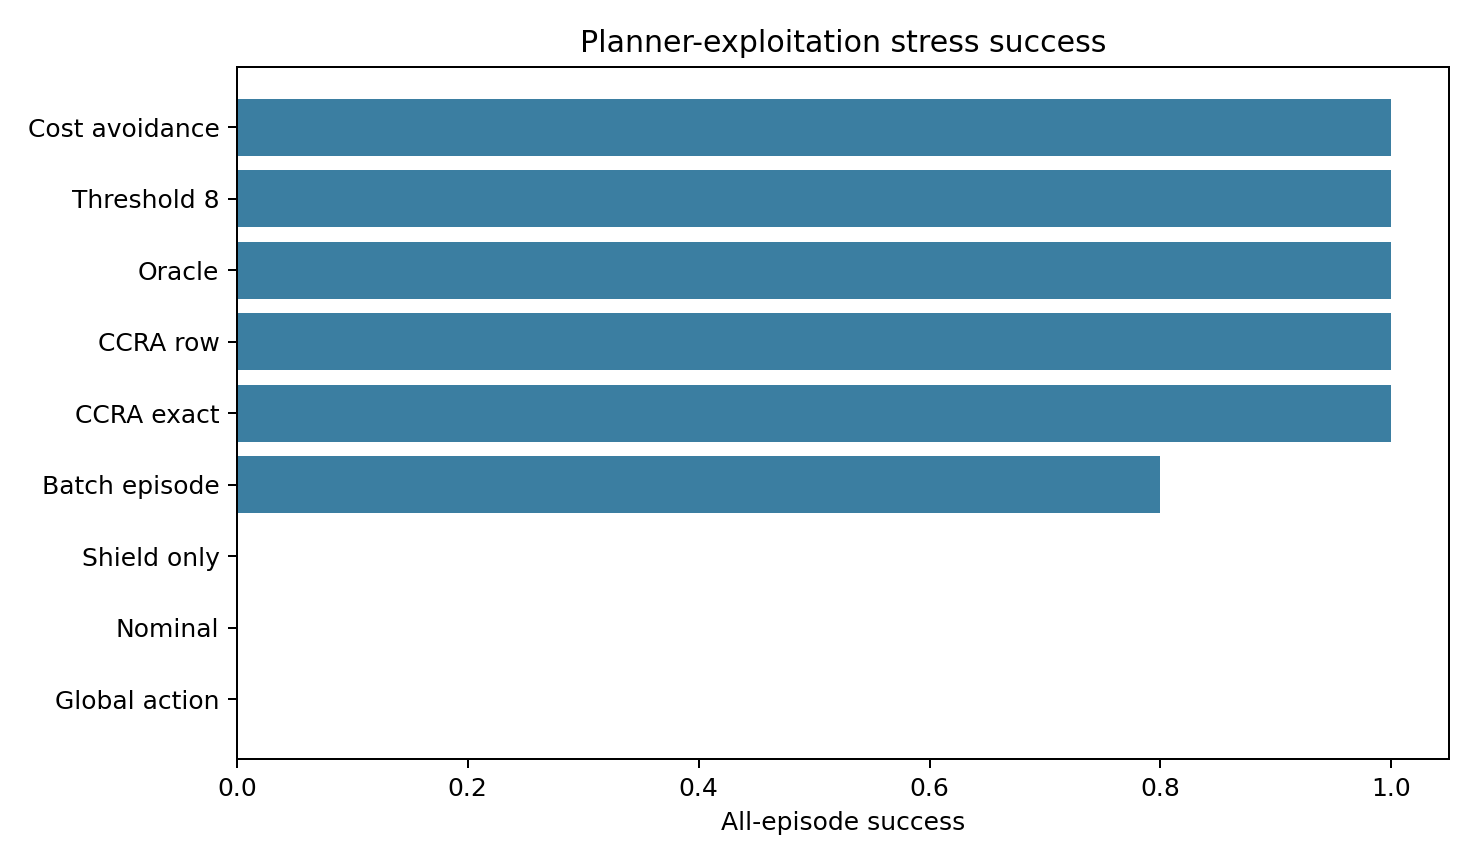
\includegraphics[width=0.92\linewidth]{figures/full_scale_success_leaderboard.png}
\caption{All-episode success in the planner-exploitation stress suite. The useful distinction is not only prediction error; it is whether the next planning call is prevented from exploiting the contradicted transition.}
\label{fig:success}
\end{figure}

\subsection{Prediction Error Can Decouple from Embodied Success}

The prediction-loss decoupling suite adds off-route faults while preserving sparse critical route faults. The nominal model has low global prediction error (0.023) but zero success. Exact CCRA reaches 1.00 success, with final prediction error 0.021 and control-weighted error 0.025. Cost avoidance also reaches 1.00 success but leaves global prediction error unchanged at 0.023. Row guards show the opposite direction: they solve many first episodes (0.97 first-episode success) but fall to 0.76 all-episode success as off-route over-blocking accumulates, with prediction error 0.085 and control-weighted error 0.333.

This suite is important because it prevents an overly simple story. Prediction error is not useless. The oracle has zero prediction error and succeeds. The point is that unweighted average error is a poor proxy for whether the planner is still authorized to use a false affordance. The scatter in Figure~\ref{fig:scatter} visualizes this: some models are globally accurate and useless for control, while others are globally less accurate but planner-useful.

\begin{figure}[t]
\centering
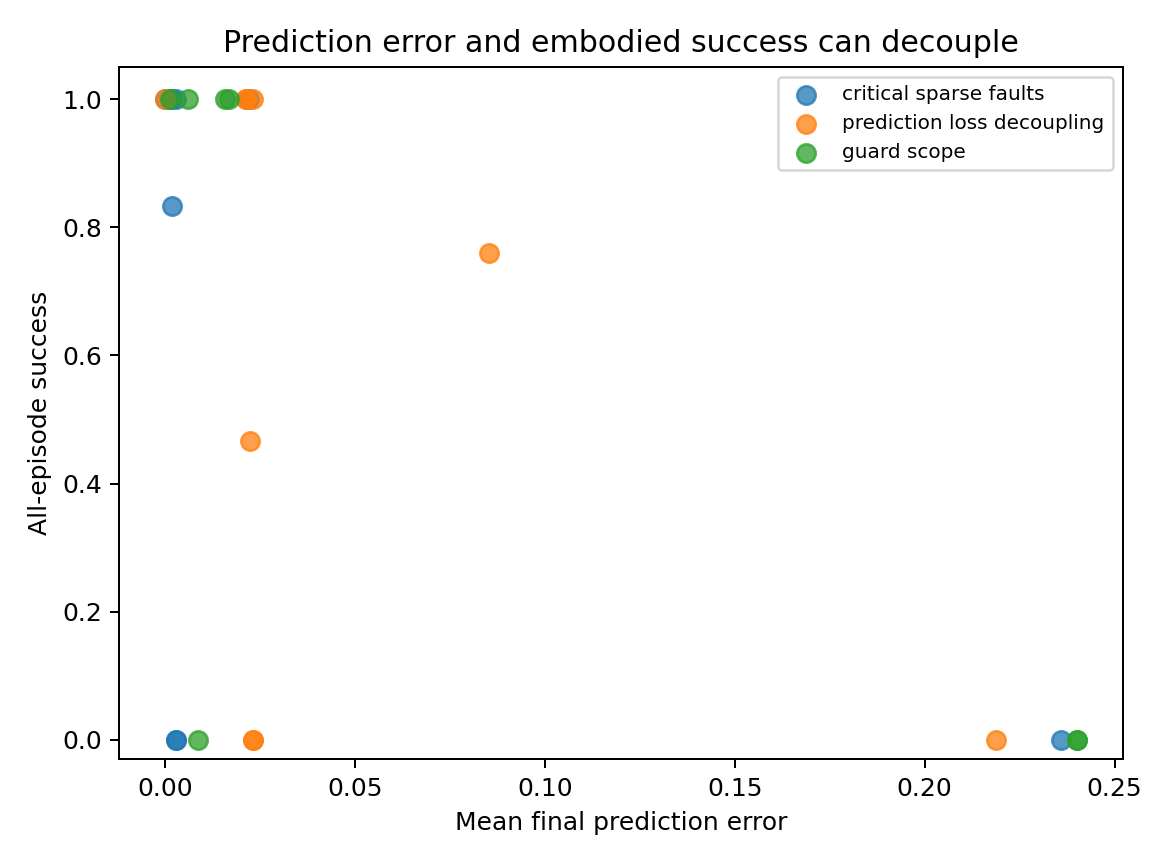
\includegraphics[width=0.82\linewidth]{figures/prediction_success_scatter.png}
\caption{Prediction error versus embodied success across key suites. The nominal model can have small average error while failing; broad guards can succeed while increasing prediction error. The paper's claim is not that prediction error never matters, but that it is not sufficient as a repair objective.}
\label{fig:scatter}
\end{figure}

\subsection{Delayed Repair Pays Counterexamples}

The threshold sweep is the most hostile ablation for novelty. It shows that exact deterministic CCRA is threshold-one blocking. The advantage is not algorithmic mystery; it is latency. In Table~\ref{tab:threshold} and Figure~\ref{fig:threshold}, threshold $k$ produces 1.00 success for all tested $k$, but first-episode counterexamples scale exactly as $1,2,4,8,16,32$. Final prediction error is the same because all thresholds eventually block the same transition. The embodied cost is paid before the model changes.

\begin{table}[t]
\centering
\small
% Auto-generated by scripts/run_full_scale_repair_loops.py
\begin{tabular}{lrrrr}
\toprule
Threshold & Success & First CE & Mean CE & Pred. err \\
\midrule
1 & 1.00 & 1.0 & 0.2 & 0.001 \\
2 & 1.00 & 2.0 & 0.4 & 0.001 \\
4 & 1.00 & 4.0 & 0.8 & 0.001 \\
8 & 1.00 & 8.0 & 1.6 & 0.001 \\
16 & 1.00 & 16.0 & 3.2 & 0.001 \\
32 & 1.00 & 32.0 & 6.4 & 0.001 \\
\bottomrule
\end{tabular}

\caption{Threshold-delay suite. Final predictive state can match across thresholds, while embodied counterexamples before repair scale with the mismatch threshold.}
\label{tab:threshold}
\end{table}

\begin{figure}[t]
\centering
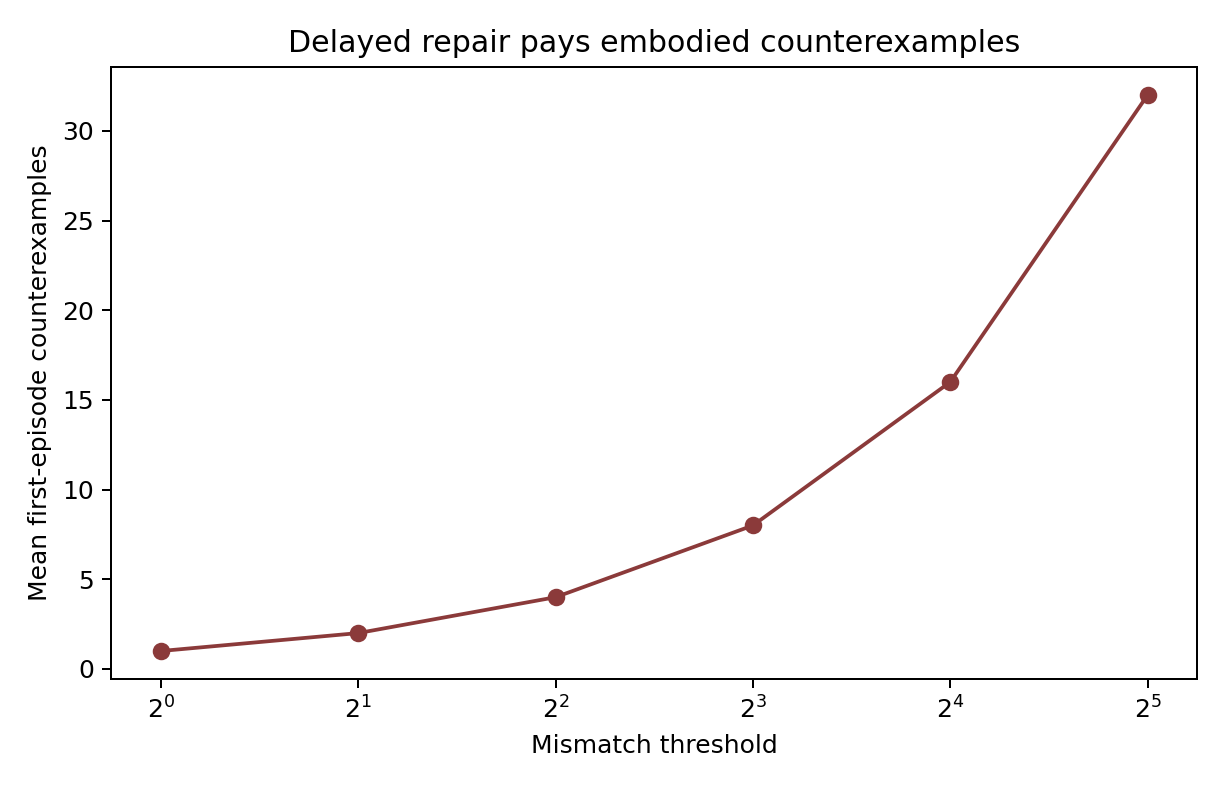
\includegraphics[width=0.72\linewidth]{figures/threshold_delay_curve.png}
\caption{Mismatch thresholds trade fewer updates for more embodied counterexamples. In this deterministic setting, exact CCRA is the threshold-one endpoint.}
\label{fig:threshold}
\end{figure}

\subsection{Guard Scope is the Main Design Frontier}

Guard scope controls the tradeoff between quick generalization and over-repair. Table~\ref{tab:guard} and Figure~\ref{fig:guard} show the scope frontier. Exact guards have perfect precision and 1.00 success, but lower recall because they only block experienced faults. Radius-1, radius-2, and row guards also reach 1.00 success, but their false-block rates rise to 0.87, 0.95, and 0.90. Column and action-wide guards fail outright in this generated family: they block too much of the reachable transition graph.

This result sharpens the paper. CCRA should not be sold as ``more repair is better.'' The patch is only useful when the guard is scoped to the physical mode it actually diagnoses. The right future work is learned guard formation from contact state, geometry, object identity, and support evidence, not broad unconditional blocking.

\begin{table}[t]
\centering
\small
% Auto-generated by scripts/run_full_scale_repair_loops.py
\begin{tabular}{lrrrrr}
\toprule
Guard & Success & Recall & Precision & False block & Pred. err \\
\midrule
CCRA exact & 1.00 & 0.51 & 1.00 & 0.00 & 0.001 \\
CCRA radius 1 & 1.00 & 0.55 & 0.13 & 0.87 & 0.006 \\
CCRA row & 1.00 & 1.00 & 0.10 & 0.90 & 0.017 \\
CCRA column & 0.00 & 0.51 & 0.08 & 0.92 & 0.009 \\
CCRA radius 2 & 1.00 & 0.57 & 0.05 & 0.95 & 0.016 \\
CCRA action & 0.00 & 1.00 & 0.01 & 0.99 & 0.240 \\
Global action & 0.00 & 1.00 & 0.01 & 0.99 & 0.240 \\
\bottomrule
\end{tabular}

\caption{Guard-scope ablation. Exact, local, and row guards can solve, but broader guards rapidly over-block. Action/global guards have high recall and near-zero precision, destroying reachability.}
\label{tab:guard}
\end{table}

\begin{figure}[t]
\centering
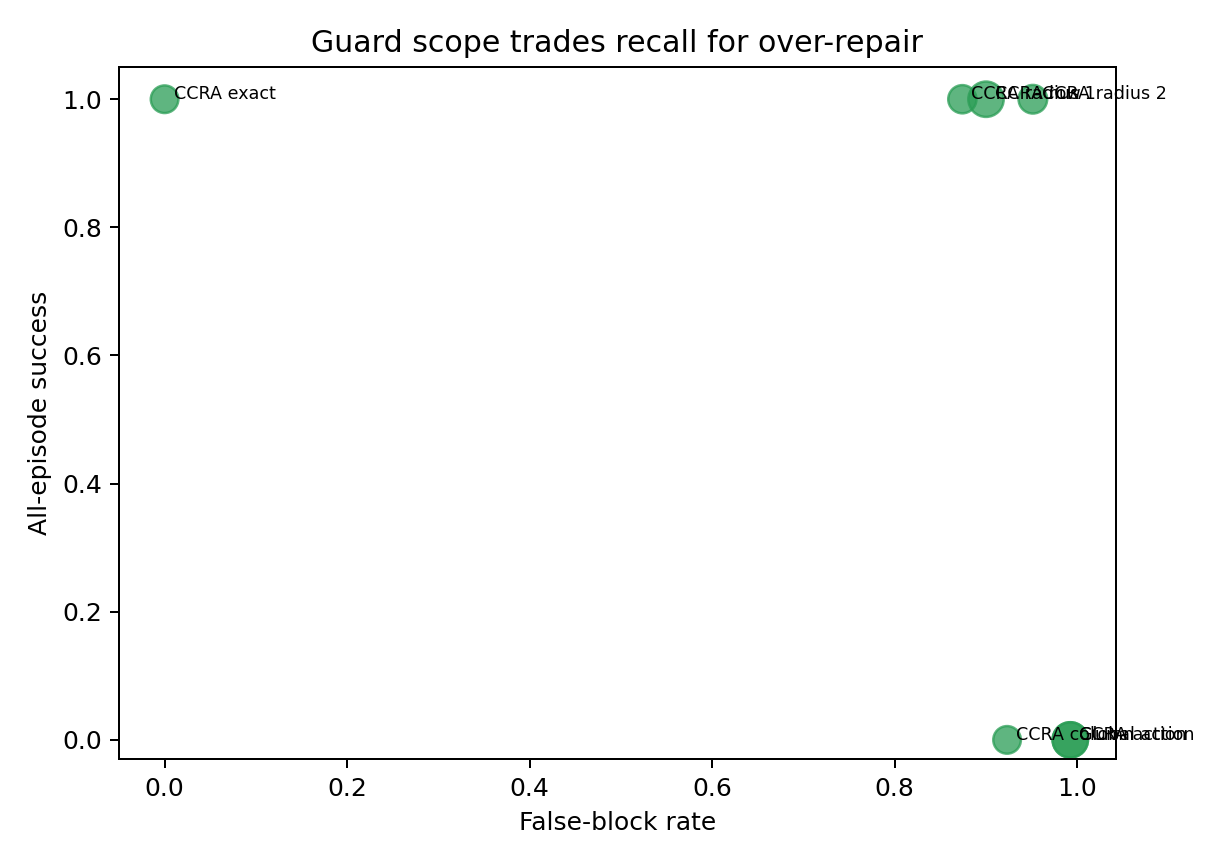
\includegraphics[width=0.78\linewidth]{figures/guard_scope_frontier.png}
\caption{Guard scope trades false-block rate against success. The marker size reflects recall. The result argues for explicit guard-scope accounting rather than unconstrained patch generalization.}
\label{fig:guard}
\end{figure}

\subsection{Stale Patches Need Retirement}

The nonstationary suite changes faults after a switch episode. Exact CCRA without retirement still succeeds, but it carries stale false blocks, producing a 0.37 false-block rate. TTL-2 retirement, TTL-4 retirement, and oracle retirement all keep success at 1.00 while reducing false blocks. TTL-2 has zero false-block rate in this suite and slightly more counterexamples because it may forget repairs that remain useful. Oracle retirement is an upper bound: it removes stale patches only when the true active fault disappears.

The result supports a practical requirement. Repair memory is not a monotonic good. A deployment system needs support counts, expiry, validation, or consolidation. Otherwise the same mechanism that prevents repeated exploitation can become a stale affordance map.

\begin{table}[t]
\centering
\small
% Auto-generated by scripts/run_full_scale_repair_loops.py
\begin{tabular}{lrrrr}
\toprule
Method & Success & False block & Pred. err & Patches \\
\midrule
CCRA exact & 1.00 & 0.37 & 0.002 & 1.2 \\
CCRA exact TTL2 & 1.00 & 0.00 & 0.001 & 0.8 \\
CCRA exact TTL4 & 1.00 & 0.07 & 0.001 & 0.9 \\
CCRA oracle retire & 1.00 & 0.00 & 0.001 & 0.9 \\
Nominal & 0.21 & 0.00 & 0.002 & 0.0 \\
Oracle & 1.00 & 0.00 & 0.000 & 0.0 \\
\bottomrule
\end{tabular}

\caption{Nonstationary retirement suite. Exact patches without retirement keep success but accumulate stale false blocks. TTL and oracle retirement reduce false-block rate while preserving success in this generated family.}
\label{tab:retirement}
\end{table}

\begin{figure}[t]
\centering
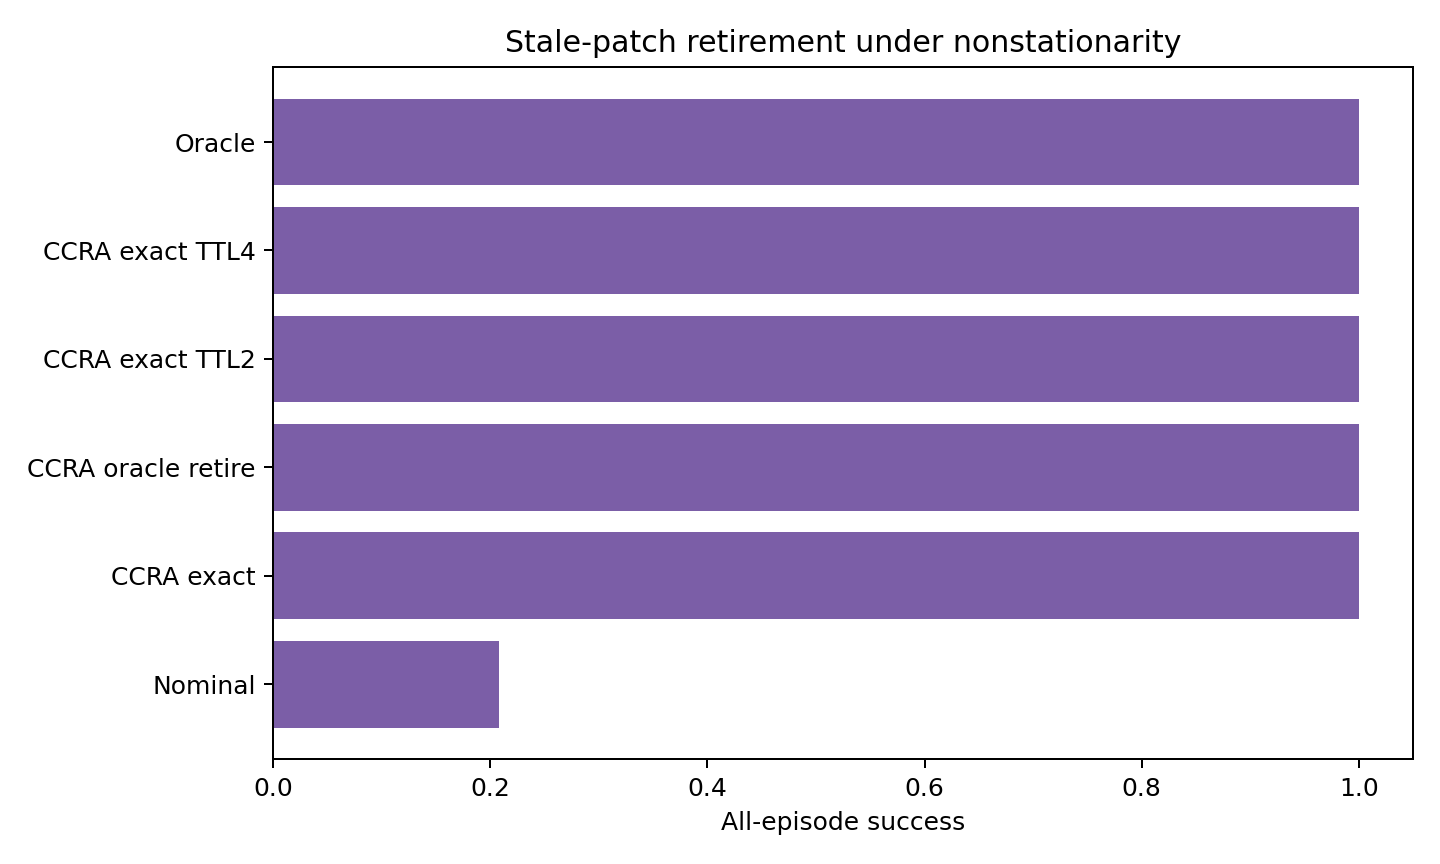
\includegraphics[width=0.82\linewidth]{figures/stale_retirement_curve.png}
\caption{Retirement variants under nonstationary faults. The mechanism needs memory hygiene; otherwise repair patches become stale model errors.}
\label{fig:retirement}
\end{figure}

\subsection{Stochastic Contradictions}

The stochastic suite makes fault edges fail with probabilities from 0.10 to 1.00. Nominal success rises above zero because a stochastic edge sometimes works, but remains poor overall at 0.26 with 154.8 counterexamples per episode. Exact CCRA, cost avoidance, thresholds, and oracle all reach 1.00 success. In this family, blocking after a contradiction is not harmful because alternative routes exist and stochastic faults lie on attractive shortcuts. Thresholds pay more counterexamples as the threshold grows. Table~\ref{tab:stochastic} and Figure~\ref{fig:stochastic} report the aggregate.

This should not be overread. In other stochastic domains, one failure may not justify a permanent block. The experiment shows that the runner can expose stochastic repair latency and false-block behavior; it does not prove a universal stochastic repair rule.

\begin{table}[t]
\centering
\small
% Auto-generated by scripts/run_full_scale_repair_loops.py
\begin{tabular}{lrrrr}
\toprule
Method & Success & CE/ep & Pred. err & False block \\
\midrule
CCRA exact & 1.00 & 0.2 & 0.001 & 0.00 \\
Cost avoidance & 1.00 & 0.2 & 0.001 & 0.00 \\
Nominal & 0.26 & 154.8 & 0.001 & 0.00 \\
Oracle & 1.00 & 0.0 & 0.001 & 0.00 \\
Threshold 2 & 1.00 & 0.4 & 0.001 & 0.00 \\
Threshold 4 & 1.00 & 0.7 & 0.001 & 0.00 \\
Threshold 8 & 1.00 & 1.3 & 0.001 & 0.00 \\
\bottomrule
\end{tabular}

\caption{Stochastic contradiction suite. In these generated maps, repair methods still reach 1.00 success because detours exist. Thresholds pay more counterexamples before repair.}
\label{tab:stochastic}
\end{table}

\begin{figure}[t]
\centering
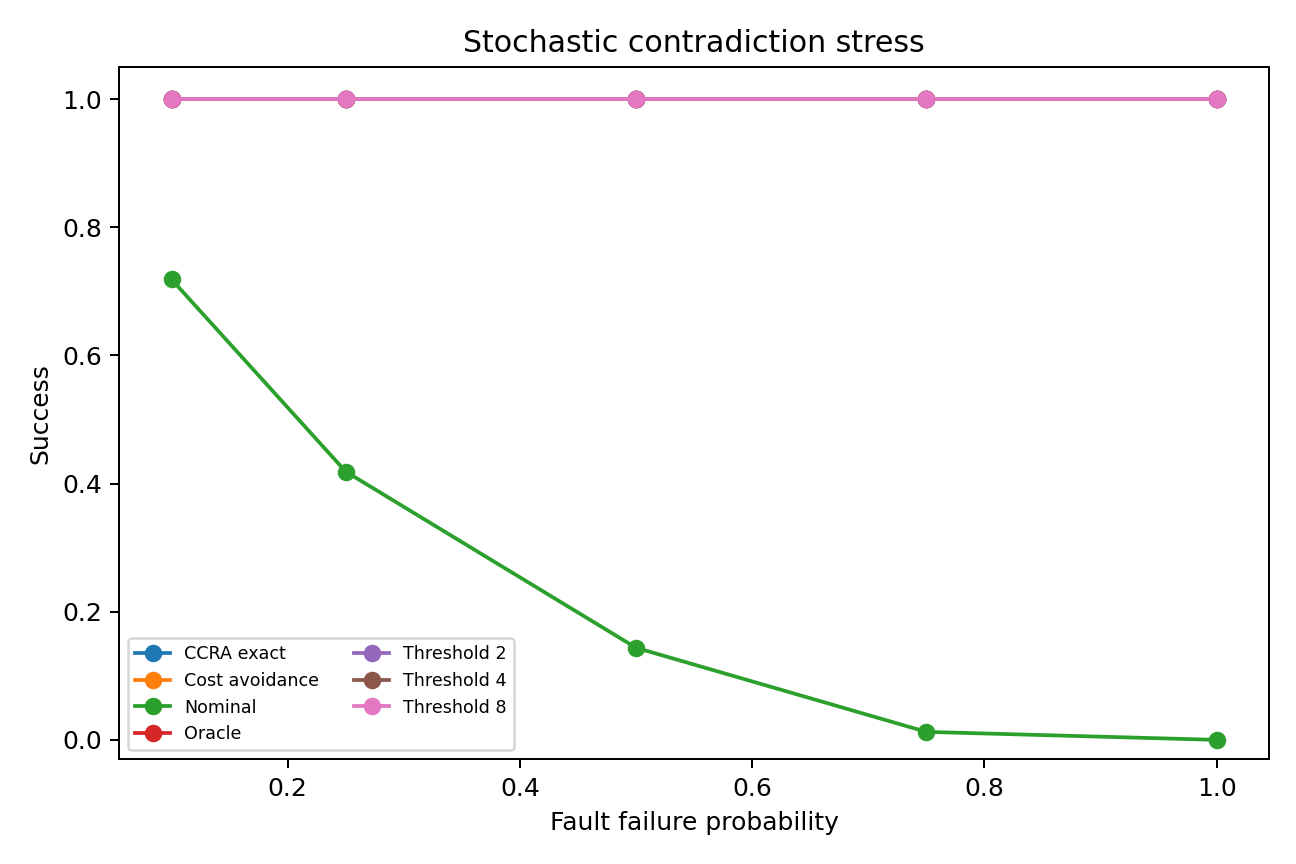
\includegraphics[width=0.82\linewidth]{figures/stochastic_success_curve.png}
\caption{Success across stochastic failure probabilities. The result is a stress diagnostic, not a theorem about stochastic safety.}
\label{fig:stochastic}
\end{figure}

\subsection{Negative Controls and Failure Cases}

Several outcomes constrain the claim.

\paragraph{Oracle success after the planner fix.}
The corrected runner uses set-based A* over known blocked transitions. This matters: an oracle that knows off-route faults should be able to weave around them when a path exists. The final corrected run has oracle success 1.00 in prediction-loss decoupling and zero prediction error. This prevents the paper from using an artificially weak oracle.

\paragraph{Broad repair can be worse than no repair.}
Global action repair has 0.00 success in critical sparse faults and planner-exploitation stress. It blocks the action class needed to reach the goal. Its false-block rate is about 0.99 and its final prediction error is about 0.24. This is a useful negative control: planner-facing repair is not automatically good.

\paragraph{Shielding is not enough when the future remains wrong.}
The shield-only baseline logs the failed action externally, but the planner's rollout still contains the false transition. It matches nominal failure in the main stress suite. This does not prove all shields fail; it shows that a shield which does not alter planning futures is not the same mechanism as transition repair.

\paragraph{Cost avoidance is a strong alternative.}
Cost avoidance solves the critical and stress suites after one counterexample. This is not embarrassing; it is evidence that the core requirement is planner-facing update, not necessarily successor replacement. A repair contract can be expressed as a transition override, an action-cost change, or an admissibility change. The manuscript uses CCRA to make the transition-patch case concrete.

\section{Discussion}

The experiments support a restrained conclusion. A world model can be globally accurate enough to look good under average prediction error and still be unusable for planning because the planner selects its rare false affordance. Conversely, a local patch can worsen global prediction error while making behavior better. The key object is the transition contract consumed by search.

The row-guard results are the cleanest example. Row guards solve the stress suite with one counterexample but introduce a 0.87 false-block rate and large control-weighted prediction error. This is not a failure of the paper; it is the design frontier. A useful repair loop must answer: what physical mode does this counterexample diagnose, and how broadly should that mode apply?

The threshold results are equally important. They strip away novelty inflation. Exact CCRA is one-mismatch blocking in the deterministic exact-guard setting. If a reviewer's complaint is ``this is just blocking the failed transition,'' the answer is yes, in this setting. The paper's claim is that this simple operation belongs in the planner-facing model and should be evaluated by embodied counterexample latency, not hidden inside eventual average prediction loss.

Finally, the stale-patch results show that repair loops need lifecycle management. A patch should carry support counts, timestamps, scope, invalidation tests, and perhaps consolidation status. If the world changes, a patch can become an error. CCRA is therefore not merely a memory cache; it is a contract with obligations and expiry conditions.

\section{Limitations}

The evidence is finite-grid simulation. It omits perception, high-dimensional sensory uncertainty, contact geometry, friction cones, compliance, dynamic manipulation, latency, and real robot hardware. The grids are designed to isolate one failure mode: sparse false transitions selected by a planner. They are not a benchmark for robot world-model performance.

The guards are hand-specified. Real embodied systems would need guard formation from sensed contact state, object geometry, proprioception, tactile observations, semantic labels, or local scene changes. The paper does not solve that learning problem. It only shows why guard scope matters and how to measure it.

The stochastic experiments are limited. They do not solve Bayesian repair, confidence calibration, risk-sensitive planning, or reversible probing. One-mismatch blocking can be too aggressive when a transition fails rarely and has no safe alternative. The appropriate repair in stochastic systems may be a cost update, probability update, confidence interval, or guarded option policy rather than a hard block.

The planner is explicit set-based A* over generated transition systems. This makes the artifact auditable but far from neural model-predictive control over images or point clouds. The paper's message should transfer as an interface requirement, not as an implementation claim.

The literature review is a broad local matrix and hostile-set synthesis, not a guarantee that every repair-like prior has been exhaustively read in full. The paper therefore avoids claiming firstness for online repair. It claims a specific framing: execution counterexamples should sometimes induce immediate planner-facing transition-contract edits, and these edits require scope, latency, and stale-memory evaluation.

\section{Conclusion}

Embodied world models should sometimes be repaired where they are used: inside the planner-facing transition relation. Counterexample-Conditioned Repair Automata are a minimal way to represent that repair. The final evidence is not hardware evidence and not a new foundation model. It is a mechanism-level stress test showing that sparse false affordances can dominate planning while barely affecting prediction error; that immediate repair prevents repeated exploitation; that delayed repair pays embodied counterexamples; that broad guards can over-repair; and that stale patches need retirement. The central update target is the transition contract the planner is allowed to believe.

\bibliography{references}
\bibliographystyle{iclr2026_conference}

\appendix
\setcounter{section}{0}
\renewcommand{\thesection}{A.\arabic{section}}

\section{Artifact Map}

The repository contains all generated evidence used in the final manuscript.
\begin{itemize}
    \item Full-scale runner: \path{scripts/run_full_scale_repair_loops.py}.
    \item Original v2 runner: \path{scripts/run_evidence.py}.
    \item Original simulator: \path{src/repair_loop_sim.py}.
    \item Full-scale rows: \path{results/full_scale/*.csv}.
    \item Full-scale summary: \path{results/full_scale/full_scale_summary.json}.
    \item Leaderboard: \path{results/full_scale/leaderboard.csv}.
    \item Paper figures: \path{paper/figures/*.png}.
    \item Paper tables: \path{paper/tables/*.tex}.
    \item Planning document: \path{docs/full_scale_execution_plan.md}.
\end{itemize}

The main regeneration commands are:
\begin{verbatim}
python scripts/smoke_test.py
python scripts/run_evidence.py
python scripts/run_full_scale_repair_loops.py --seed-scale 20
python scripts/run_full_scale_repair_loops.py --summarize-only
\end{verbatim}

\section{RAM-Light Execution}

The full-scale runner writes one compact CSV row per episode. It does not retain raw trajectories. Each suite is generated sequentially. The script computes blocked-transition sets from the current patch state, derives prediction metrics from those sets and active faults, and streams rows to disk. The completed corrected run used 34,880 per-episode rows and stayed around 60 MB of working memory in local monitoring.

The first attempted full pass used a row-only planner. That was rejected because the oracle could underperform in off-route-noise settings: it knew many faults but could not weave around them. The final runner uses set-based A* over known blocked transitions, so oracle planning is a valid upper bound in these generated grids.

\section{Baseline Details}

\paragraph{Nominal.}
The nominal model always predicts ordinary grid transitions. It never updates. It is the cleanest demonstration that low global prediction error can coexist with repeated exploit failures.

\paragraph{Shield only.}
The shield-only baseline records that an executed state-action pair failed and blocks it at execution time, but it does not change the planner's rollout model. This represents a detached safety layer that does not rewrite the future searched by the planner.

\paragraph{Batch episode.}
The batch learner records mismatches during an episode and commits exact blocks only after the episode ends. It shows why repair timing matters: it can eventually improve later episodes while still failing the first episode.

\paragraph{Threshold repair.}
Threshold repair blocks an exact state-action transition after $k$ mismatches. In deterministic repeated-exploit settings, first-episode counterexamples scale with $k$.

\paragraph{Cost avoidance.}
Cost avoidance adds planner cost to a contradicted transition. It is planner-facing but does not change the predicted successor. Its strong performance shows that the general requirement is to alter what planning will choose, not necessarily to store a hard transition replacement in every domain.

\paragraph{CCRA exact.}
Exact CCRA immediately blocks the contradicted state-action pair. It is conservative and high precision, but it may need many observations if faults recur across a mode.

\paragraph{Broad CCRA guards.}
Row, column, radius, and action guards generalize a mismatch. They are useful for measuring over-repair. In these grids, row and radius guards can solve, but action-wide and global action guards destroy reachability.

\paragraph{Oracle.}
The oracle knows active true blocked transitions. It plans with the same set-based A* planner as other baselines but with the true blocked set. It is not a robot-realistic method; it is a correctness upper bound.

\section{Suite Definitions}

\paragraph{Critical sparse faults.}
This suite varies grid width and the number of on-route faults. It checks whether the original sparse-fault mechanism survives larger route lengths and multiple false affordances.

\paragraph{Prediction-loss decoupling.}
This suite adds off-route rightward faults. These faults affect global prediction error but may not affect the current best route. The suite tests whether global prediction error, control-weighted prediction error, and success can disagree.

\paragraph{Threshold delay.}
This suite sweeps exact mismatch thresholds. It is designed to be hostile to novelty: threshold-one is exact CCRA in deterministic exact-guard settings.

\paragraph{Guard scope.}
This suite compares exact, local, row, column, action, and global scopes. It reports success, recall, precision, false-block rate, and prediction error.

\paragraph{Nonstationary retirement.}
Faults are removed, moved, or added after a switch episode. The suite tests whether stale patches remain harmful and whether TTL retirement can reduce false blocks.

\paragraph{Stochastic contradictions.}
Faults fail probabilistically. The suite tests whether one-mismatch repair and threshold repair behave sensibly when contradictions are not deterministic.

\paragraph{Planner-exploitation stress.}
This suite uses the largest grids and fault counts. It is the main aggregate stress table in the paper.

\section{Metric Definitions}

Let $B_t$ be the set of transitions blocked by a model at episode $t$, and let $F_t$ be the active true fault set. In deterministic suites, global prediction error is proportional to transitions in the symmetric difference between $B_t$ and $F_t$ plus any unblocked faults. In stochastic suites, each fault contributes its failure probability when unblocked and one minus that probability when blocked.

Guard precision is $|B_t\cap F_t|/|B_t|$ when $B_t$ is nonempty. Guard recall is $|B_t\cap F_t|/|F_t|$ when $F_t$ is nonempty. False-block rate is $|B_t\setminus F_t|/|B_t|$. Control-weighted prediction error uses larger weights for route-critical rightward transitions than for off-route transitions. These weights are diagnostic rather than normative.

\section{Original v2 Evidence}

The original evidence remains reproducible through \path{scripts/run_evidence.py}. It uses 80 seeded sparse-contact grid worlds with five deployment episodes per method. Nominal no-repair has 0.00 first-episode success and 114.6 first-episode counterexamples with final prediction error 0.004. Exact CCRA reaches 1.00 first-episode success with 1.0 counterexample. Row-guard CCRA also reaches 1.00 success with 1.0 counterexample while worsening final prediction error to 0.022. The v2 threshold sweep shows thresholds 1, 2, 4, 8, and 16 paying exactly that many first-episode counterexamples.

The v3 run supersedes this evidence in scale but not in direction. It preserves the narrow interpretation: exact CCRA is threshold-one blocking in the deterministic exact-guard case.

\section{Additional Result Interpretation}

\paragraph{Why batch episode reaches 0.80 in stress.}
Batch episode repair fails first episodes because it does not update the planner-facing model until the episode ends. Later episodes can improve because exact blocks are committed. Its 0.80 all-episode success in the stress suite therefore reflects delayed repair, not immediate embodied recovery.

\paragraph{Why row guards can solve and still be bad.}
In the generated corridor maps, blocking the middle row often forces a detour that works. This explains 1.00 success for row guards in the stress suite. But row guards also block many valid transitions, producing false-block rates near 0.9 and high control-weighted error. The result argues for reporting both success and repair precision.

\paragraph{Why cost avoidance is included.}
Cost avoidance is a strong baseline because it changes planner choice without transition replacement. It is evidence against a too-narrow claim that only transition patches can work. The more general requirement is planner-facing repair; CCRA is one explicit representation of that requirement.

\paragraph{Why global action repair fails.}
Global action repair overgeneralizes from rightward faults to the entire rightward action class. Because rightward motion is needed to reach the goal, this destroys reachability. This is the simplest failure case for broad guard scope.

\section{Guard-Scope Design Notes}

A deployment-quality repair guard should answer at least five questions:
\begin{enumerate}
    \item What sensed variables were present when the contradiction occurred?
    \item Which variables are causal for the failed transition rather than incidental?
    \item How much support is required before a broad guard is installed?
    \item What validation can falsify the guard later?
    \item How does the planner behave if the guard makes the task unreachable?
\end{enumerate}

Exact guards answer these questions conservatively: they only bind the observed state-action pair. Broad guards need stronger evidence. In robotics, the right guard might involve contact mode, object identity, local geometry, gripper condition, friction estimate, or recent tactile history. The present simulator does not learn such guards. It only shows that guard scope is measurable and consequential.

\section{Stale Patch Lifecycle}

Repair patches are useful because they remember contradictions. They are dangerous because the world changes. A patch installed when an object is wedged may become stale after the object moves. A patch installed when a wheel slips may become stale after the robot leaves the surface. A patch installed when a gripper finger is saturated may become stale after unloading.

The nonstationary suite implements a minimal version of this issue. Faults can be removed, moved, or added after a switch episode. Exact CCRA without retirement keeps success but accumulates false blocks. TTL retirement reduces stale memory at the cost of possible re-observation. Oracle retirement is an upper bound. A real system would need support decay, validation probes, consolidation into a better model, or context-sensitive expiry.

\section{Relationship to Dyna and Planning Updates}

Dyna-style architectures integrate learning, planning, and acting \citep{sutton1991dyna}. CCRA is compatible with that view but emphasizes a specific update object: a planner-facing transition patch induced by an execution counterexample. The patch can be used immediately for planning even before broader model learning. This does not make CCRA more general than Dyna; it identifies a small repair contract that Dyna-like systems should expose and evaluate when sparse false affordances dominate behavior.

\section{Relationship to Shields}

Shields can prevent unsafe actions \citep{alshiekh2018shielding}. A shield may be enough if the task only needs one-step action filtering. The distinction studied here is multi-step rollout. If the planner continues to believe the false future, it may return plans that depend on the same affordance. A planner-facing patch makes the future searched by the planner different. The shield-only baseline is intentionally narrow; it should not be read as a rejection of all shielding approaches.

\section{Relationship to Online System Identification}

Online system identification estimates hidden variables or parameters that explain deployment dynamics \citep{yu2017uposi}. That is powerful when a low-dimensional parameter controls the mismatch. CCRA covers a different local case: the repair may be a discontinuous forbidden affordance with no compact global parameter. The two mechanisms can be combined. A CCRA patch can provide immediate safety and task recovery while a slower system-identification module infers a broader cause.

\section{Reproducibility Checklist}

The final artifact should satisfy:
\begin{itemize}
    \item v2 smoke test and evidence run reproduce.
    \item v3 full-scale runner executes with \path{--seed-scale 20}.
    \item \path{--summarize-only} regenerates tables and figures from existing CSVs.
    \item \path{results/full_scale/full_scale_summary.json} reports 34,880 rows.
    \item Generated figures are copied to \path{paper/figures}.
    \item Generated tables are copied to \path{paper/tables}.
    \item Final PDF is built only after the manuscript clears the page gate.
    \item The final numbered PDF is copied only after the local build is verified as the actual paper.
\end{itemize}

\section{Claim Audit}

Supported claims:
\begin{itemize}
    \item Sparse planner-attractive false transitions can dominate task success while barely affecting average prediction error in the implemented transition systems.
    \item Immediate planner-facing repair prevents repeated exploitation in deterministic exact-guard settings.
    \item Thresholded repair trades update conservatism for embodied counterexamples.
    \item Guard scope creates a measurable precision/recall/false-block frontier.
    \item Stale patches require retirement or validation.
\end{itemize}

Unsupported claims:
\begin{itemize}
    \item Real-robot performance.
    \item Learned visual or tactile guard formation.
    \item High-dimensional continuous-control scalability.
    \item General stochastic safety.
    \item Novelty over all forms of online adaptation, shielding, or model reconciliation.
\end{itemize}

\section{Baseline Mechanism Table}

Table~\ref{tab:baseline_access} records what each baseline is allowed to change. This table is included because many apparent disagreements about the paper reduce to interface access. A method that only changes a detached log is not comparable to a method that changes planner rollouts. A method that changes cost but not successor prediction can still be planner-facing. A method that changes an entire action class is planner-facing but too broad.

\begin{table}[h]
\centering
\small
% Auto-generated by scripts/run_full_scale_repair_loops.py
\begin{tabular}{lrrr}
\toprule
Baseline & Planner-facing update & Generalizes & Retires \\
\midrule
Nominal & No & No & No \\
Shield only & No transition rewrite & No & No \\
Batch episode & After episode & Exact & No \\
Threshold & After k mismatches & Exact & No \\
Cost avoidance & Cost only & Exact & No \\
CCRA exact & Immediate transition patch & Exact & No \\
CCRA row & Immediate transition patch & Row & No \\
Global action & Immediate broad patch & Action & No \\
Oracle & True transition model & True faults & Yes \\
\bottomrule
\end{tabular}

\caption{Interface access of baselines. The experiments separate detached shielding, delayed batch update, thresholded exact update, immediate exact CCRA, broader guard CCRA, and oracle access.}
\label{tab:baseline_access}
\end{table}

\section{Corrected Planner Audit}

The full-scale pass went through an explicit audit before being used in the manuscript. The first scalable implementation used a corridor planner: it searched for one row from the current state to the goal and then moved horizontally along that row. This was fast and matched the original simple route, but it created a methodological problem in the prediction-loss decoupling suite. When many off-route faults were added, the oracle knew too many blocked transitions. The row-only planner could declare failure if no single row had a completely clear rightward path, even though a path existed by weaving between rows. A less-informed CCRA model could appear to outperform the oracle because it had not yet discovered all off-route faults. That is not an acceptable upper bound.

The corrected runner therefore uses set-based A* over the grid. At each planning call, the model is converted into a set of currently blocked transitions. The planner then searches over all legal moves, skipping blocked transitions and adding model-specific action costs. This preserves the speed advantage of precomputed blocked sets while allowing the oracle and repaired models to route around known faults. After this correction, the oracle reaches 1.00 success in the prediction-loss decoupling suite with zero prediction error. The final manuscript uses only the corrected run.

This audit matters beyond this artifact. A planner-facing repair paper can easily produce misleading results if the planner is not held fixed or if the oracle is accidentally weaker than a learning method. The final implementation treats the planner as shared infrastructure and varies only the model interface: no repair, detached shield, delayed update, cost update, exact patch, broad patch, or oracle blocked set.

\section{Metric Derivations}

For each generated grid, let $K$ be the set of all state-action transitions considered by the prediction metric. Let $F_t\subseteq K$ be the active true fault set in episode $t$, and let $B_t\subseteq K$ be the set of transitions blocked by the planner-facing model. In deterministic suites, a nominal unblocked transition is correct for $k\notin F_t$ and wrong for $k\in F_t$. A blocked transition is correct for $k\in F_t$ and wrong for $k\notin F_t$. Thus the unweighted prediction error is
\[
    \ell_t(B_t,F_t)=\frac{|F_t\setminus B_t|+|B_t\setminus F_t|}{|K|}.
\]
This formula is useful because it makes the decoupling mechanism visible. If $|K|$ is large and $|F_t|$ is small, the nominal model can have a tiny $\ell_t$ even when the fault lies on the only route the planner wants. If a broad guard blocks a row, $|B_t\setminus F_t|$ can become large, increasing prediction error while still improving task success.

For stochastic suites, each active fault $k\in F_t$ fails with probability $p$. If the model does not block $k$, the expected one-step prediction error contribution is $p$. If the model blocks $k$, the contribution is $1-p$ because the edge sometimes would have succeeded. For inactive transitions blocked by the model, the contribution is 1. The runner computes this expectation directly rather than sampling prediction-error estimates from rollouts.

The control-weighted error uses the same terms but replaces the uniform denominator with a weighted one. Route-critical rightward transitions on the shortest row receive the largest weight; nearby rightward transitions receive smaller elevated weight; all other transitions receive weight one. The exact weights are not meant as a universal robotics objective. They are a diagnostic that moves the prediction metric toward the planner's sampling distribution.

Guard precision, recall, and false-block rate are:
\[
    \text{precision}=\frac{|B_t\cap F_t|}{|B_t|},\quad
    \text{recall}=\frac{|B_t\cap F_t|}{|F_t|},\quad
    \text{false-block}=\frac{|B_t\setminus F_t|}{|B_t|}.
\]
When the denominator is zero, the runner uses the benign convention of precision or recall equal to one if there is nothing to block or recall. The main reported false-block rates occur for nonempty blocked sets.

\section{Suite-by-Suite Numeric Audit}

\paragraph{Critical sparse faults.}
This suite is the scaled version of the original phenomenon. Nominal and shield-only have 0.00 success and 171.9 first-episode counterexamples despite final prediction error 0.0028. Exact CCRA succeeds with 1.0 first-episode counterexample and final prediction error 0.0016. Threshold-8 succeeds but pays 8.0 first-episode counterexamples. Batch episode reaches 0.833 all-episode success because later episodes benefit from committed repairs, but first episodes still fail. Row guard succeeds with one counterexample but has a 0.889 false-block rate and control-weighted error 0.3047. Global action repair fails because it blocks the action needed for progress.

\paragraph{Prediction-loss decoupling.}
Off-route faults increase global prediction error. Nominal still fails with 0.00 success, 171.0 first-episode counterexamples, and prediction error 0.0231. Exact CCRA reaches 1.00 success with 2.72 first-episode counterexamples and prediction error 0.0214. Cost avoidance reaches 1.00 success while leaving prediction error at 0.0231. Row guard first-episode success is high at 0.97, but all-episode success drops to 0.76 because broad patches collide with off-route faults and detours. This is the suite where the corrected oracle matters: it now reaches 1.00 success with zero prediction error.

\paragraph{Threshold delay.}
Thresholds 1, 2, 4, 8, 16, and 32 all reach 1.00 success. Their first-episode counterexamples are exactly 1.0, 2.0, 4.0, 8.0, 16.0, and 32.0. Mean counterexamples per episode are one fifth of those values because five episodes are run and the model persists. Final prediction error is constant at 0.0012 because the same exact transitions are eventually blocked. This is the strongest support for the latency framing.

\paragraph{Guard scope.}
Exact guards succeed with zero false blocks. Radius-1 and radius-2 guards also succeed but have false-block rates 0.874 and 0.951. Row guards succeed with false-block rate 0.900. Column guards fail with 0.00 success even though their prediction error is not as large as action-wide repair; they block structurally important vertical slices. Action/global guards fail with false-block rate 0.992 and prediction error 0.240. The suite shows that guard recall alone is dangerous: action-wide guards have recall 1.00 but almost no precision.

\paragraph{Nonstationary retirement.}
Nominal has 0.208 all-episode success because in some switched episodes faults disappear or move in a way that helps. Exact CCRA, TTL-2, TTL-4, oracle-retire, and oracle all have 1.00 success. The difference is stale memory: exact CCRA without retirement has false-block rate 0.37, TTL-4 has 0.07, and TTL-2 and oracle-retire have 0.00. TTL-2 pays more counterexamples per episode because useful patches expire sooner. This is the patch lifecycle tradeoff.

\paragraph{Stochastic contradictions.}
Nominal reaches 0.259 success because probabilistic faults sometimes allow the route through, but it still pays 154.8 counterexamples per episode. Exact CCRA reaches 1.00 success with 0.17 counterexamples per episode. Threshold 2, 4, and 8 also reach 1.00 success while paying 0.37, 0.72, and 1.28 counterexamples per episode. Oracle has 1.00 success. In this generated family, one-mismatch blocking is not harmful because detours exist and faults are planner-attractive. The limitation remains: other stochastic tasks may require probabilistic repair rather than hard blocking.

\paragraph{Planner-exploitation stress.}
This is the headline stress suite. Nominal and shield-only fail completely with 252.3 first-episode counterexamples. Exact CCRA and cost avoidance solve after 1.0 first-episode counterexample. Threshold-8 solves after 8.0. Batch episode reaches 0.80 all-episode success but fails first episodes. Row guard solves but carries false-block rate 0.874 and control-weighted error 0.2641. Global action repair fails.

\section{Failure Catalog}

The experiments produce a small but useful failure taxonomy.

\paragraph{Repeated exploit failure.}
The planner returns to the same false edge after execution contradicts it. Nominal and shield-only baselines exhibit this failure. The symptom is high counterexamples, low success, and low prediction error. The repair is to make the contradiction planner-facing.

\paragraph{Delayed repair failure.}
The system has enough evidence to repair but waits for a threshold or episode boundary. Threshold and batch baselines show this. The symptom is eventual success but high first-episode counterexamples. The repair is to lower latency or distinguish high-consequence contradictions from low-consequence noise.

\paragraph{Over-broad guard failure.}
A patch generalizes beyond the physical mode that caused the contradiction. Row guards show a mild version; action-wide and global action repair show a severe version. The symptom is high false-block rate, high control-weighted error, or unreachable plans. The repair is better guard learning, support tests, and fallback planning.

\paragraph{Stale patch failure.}
A patch remains after the world changes. Exact CCRA without retirement in the nonstationary suite shows this: success stays high, but false-block rate rises. The repair is TTL, support decay, validation probing, or consolidation into a model that can be invalidated.

\paragraph{Prediction-objective failure.}
The model has low average prediction error but fails control. Nominal in the stress suites shows this. The repair is not simply to report another prediction number; it is to evaluate whether the planner-facing contract changes after embodied counterexamples.

\paragraph{Planner-upper-bound failure.}
The initial row-only planner caused oracle underperformance. This is not a robot failure; it is an evaluation failure. The repair was to use a shared set-based A* planner for all methods and rerun the evidence. This failure is included because it is exactly the kind of artifact bug that can make a paper look stronger than it is.

\section{Implementation Details}

The full-scale runner is self-contained except for Matplotlib figure generation. Environment generation is deterministic by seed. All faults are represented as transition keys $((x,y),a)$. The nominal step function checks grid boundaries. The true step function returns the original state on a fault with the configured fault probability. The planner converts the model's current patches into blocked transition keys, then runs A* over the grid. For cost-avoidance models, blocked keys remain empty but edge costs increase on contradicted transitions.

Loop detection prevents slow repeated failures. If an episode reaches the same state with the same planner-facing model signature, the runner counts the remaining steps as repeated counterexamples and returns failure. For batch episode repair, pending observations are excluded from the signature because they do not change planning until the episode ends. This is important: otherwise the simulator would waste time replaying a known doomed loop even though the planner-facing model has not changed.

The generated CSV rows contain suite name, config id, seed, strategy, episode, grid size, fault counts, success, steps, mismatches, replans, shield blocks, repeated-loop flag, patch count, final prediction error, final control-weighted error, blocked key count, guard true positives, guard false positives, precision, recall, and false-block rate. This is enough to regenerate all tables and figures without raw trajectories.

\section{Why Not Just Add More Learning?}

A natural objection is that a sufficiently good learned world model would not need patches. That may be true in some deployments. The point here is about timing and interface. A robot often needs the next plan to avoid the just-observed contradiction before a global learner has converged. The patch is an immediate operational object. It can later be consolidated into a learned model, used as replay data, or turned into a simulator parameter update.

Another objection is that model-based control already evaluates task success. Many papers do. The paper's narrower claim is that the update object is often still prediction-centric: new data improves a predictor, updates a latent, adjusts a parameter, or calibrates uncertainty. CCRA asks whether the specific transition relation used in search has been changed so the same exploit is not available. Task success evaluation and planner-facing repair are complementary.

\section{How This Would Extend to Robots}

In a contact-rich robot system, a state-action guard would not be a grid coordinate. It might bind to a local contact patch, an object pose relation, a gripper aperture range, a force threshold, a tactile slip signature, a tool frame, or a semantic affordance. A replacement transition might say that a push leaves the object wedged, that a grasp closes without lifting, or that a navigation action saturates against a surface. A broad guard might generalize across neighboring contact patches or similar object poses. A stale-patch test might probe whether the contact has cleared.

The core interface remains the same. The patch must be visible to the planner. If the planner imagines futures using a neural latent model, then the patch may be a constraint or residual applied during latent rollout. If the planner searches a symbolic abstraction, the patch may be a deleted precondition or blocked effect. If the planner uses sampling-based MPC, the patch may be a cost or transition override in the rollout simulator. The paper's grid artifact is a minimal model of this interface.

\section{Reviewer Attack Responses}

\paragraph{``This is just one-mismatch blocking.''}
Yes, for deterministic exact guards. The manuscript states this and uses the threshold sweep to quantify it. The contribution is the planner-facing repair obligation and the metrics around latency, scope, and stale memory.

\paragraph{``Prediction loss is a strawman.''}
The paper does not claim that robotics papers ignore task success. It claims that average prediction error can be a poor update target when the planner repeatedly exploits sparse false transitions. The experiments include task success, counterexamples, prediction error, and control-weighted error together.

\paragraph{``Cost avoidance solves the same problem.''}
In several suites it does. That strengthens the broader interface claim: the planner-facing contract can be repaired by transition replacement, cost change, or admissibility change. CCRA is one explicit transition-patch representation.

\paragraph{``Broad patches overfit.''}
Correct. The guard-scope and nonstationary suites exist to show this. The paper argues for explicit scope and lifecycle accounting, not unbounded repair memory.

\paragraph{``The evidence is toy.''}
Correct. It is a mechanism paper. The simulator is deliberately simple enough to make the failure mode, planner interface, and metrics auditable. Hardware and high-fidelity simulation are future work, not hidden claims.

\section{Extended Claim Boundary}

The final claim can be stated in one sentence: when execution contradicts a transition that a robot planner was relying on, the next model update should sometimes be a scoped planner-facing repair of that transition contract, and its quality should be evaluated by repeated-exploit prevention, repair latency, guard scope, and stale-memory behavior, not only by average prediction error.

Every phrase in that sentence matters. ``Sometimes'' excludes universal claims. ``Execution contradicts'' excludes purely imagined errors. ``Planner was relying on'' excludes irrelevant model mistakes. ``Scoped'' excludes action-wide overblocking. ``Planner-facing'' excludes detached logs. ``Transition contract'' allows transition, cost, or admissibility changes. ``Not only'' keeps prediction quality in the evaluation rather than discarding it.

\section{Concrete Counterexample Construction}

The smallest deterministic construction behind the paper can be written without any grid machinery. Let the state space contain start $s_0$, shortcut state $s_1$, detour states $d_1,\ldots,d_m$, and goal $g$. The nominal model has action $a$ from $s_0$ to $s_1$ and action $b$ from $s_1$ to $g$. The true environment makes $b$ a self-loop at $s_1$. A detour action sequence from $s_0$ through $d_1,\ldots,d_m$ reaches $g$. A shortest-path planner under the nominal model selects $a,b$ because it is shorter than the detour. Execution reaches $s_1$, executes $b$, and stays in $s_1$.

If the model is not repaired, replanning at $s_1$ selects $b$ again. The transition table has one wrong entry out of many possible entries. Average error can be made arbitrarily small by adding irrelevant states and correct transitions. Yet task success is zero under a step cap because the planner repeatedly selects the attractive false edge.

An exact patch that maps $(s_1,b)$ to $s_1$ removes the false edge from the planner's useful graph. A cost patch that makes $(s_1,b)$ expensive can also work if the detour is cheaper after the cost increase. A row-like broad patch can work if it blocks a set of shortcut edges and leaves a detour. An action-wide patch fails if it blocks the action needed for the detour. This toy graph explains all main empirical outcomes in miniature:
\begin{itemize}
    \item nominal failure with low prediction error;
    \item exact repair after one counterexample;
    \item threshold delay with $k$ counterexamples;
    \item cost repair as an alternative planner-facing contract;
    \item broad repair helping or destroying reachability depending on scope;
    \item stale repair when the true edge later becomes valid again.
\end{itemize}

The grid experiments are useful because they instantiate this graph in many configurations, with multiple faults, off-route noise, stochastic outcomes, and nonstationarity. But the core mechanism is already present in this finite construction.

\section{CSV Schema and Auditability}

Each full-scale row is deliberately flat. The fields are:
\begin{itemize}
    \item \path{suite}: experimental suite name.
    \item \path{config_id}: parameter configuration within the suite.
    \item \path{env_label}: human-readable environment label.
    \item \path{seed}: deterministic environment seed.
    \item \path{strategy} and \path{display}: machine and display names for the baseline.
    \item \path{episode}: deployment episode index for a persistent model.
    \item \path{width}, \path{height}, \path{fault_count}, \path{active_fault_count}, \path{offroute_fault_count}, and \path{fault_probability}: environment descriptors.
    \item \path{switch_episode}: nonstationary switch point when applicable.
    \item \path{success}, \path{steps}, \path{mismatches}, \path{replans}, \path{shield_blocks}, and \path{repeated_loop}: episode outcomes.
    \item \path{patch_count}: number of committed planner-facing patches or equivalent memory items.
    \item \path{final_prediction_error} and \path{final_control_weighted_error}: global and control-weighted model errors after the episode.
    \item \path{blocked_key_count}, \path{guard_true_positive}, \path{guard_false_positive}, \path{guard_precision}, \path{guard_recall}, and \path{false_block_rate}: repair-scope diagnostics.
\end{itemize}

This schema is intentionally not optimized for storage. It is optimized for review. A reader can group by suite and strategy, recompute the leaderboard, or inspect failure cases with ordinary CSV tools. The \path{--summarize-only} mode performs exactly that operation: it reads the existing CSVs, regenerates \path{leaderboard.csv}, writes \path{full_scale_summary.json}, rewrites the LaTeX tables, and redraws the PNG figures.

\section{Rejected Design Alternatives}

\paragraph{Only reporting task success.}
Task success alone would make exact CCRA, row CCRA, threshold repair, and cost avoidance look similarly good in some suites. That would hide the difference between precise repair, delayed repair, over-broad repair, and cost-only repair. The final paper reports counterexamples, prediction error, control-weighted error, precision, recall, and false-block rate so these mechanisms cannot collapse into one success number.

\paragraph{Only reporting prediction error.}
Prediction error alone would miss the central failure. Nominal can have lower global prediction error than a successful row-guard model. It can also have low prediction error while failing every episode. Prediction error remains in the paper, but it is not allowed to be the only objective.

\paragraph{Using a learned neural model in this pass.}
A neural model would make the artifact less transparent and would introduce training instability, hyperparameters, and hardware/runtime variation. The chosen finite transition systems make the repair contract exactly inspectable. A future version can place the same interface around a learned latent model, but this paper first isolates the mechanism.

\paragraph{Using a detached verifier as the main method.}
A verifier can reject an action at execution time, but if it does not change the planner's future rollout, the planner can keep proposing futures that depend on the false transition. The shield-only baseline captures this distinction. More sophisticated shields that feed constraints back into planning would count as planner-facing repair under the broader framing.

\paragraph{Using only an oracle.}
The oracle is necessary as an upper bound, but it is not a repair method. It does not show how counterexamples should update a model. The corrected oracle is included to make sure learned or patched methods do not benefit from an artificially weak planner.

\section{Robot Extension Protocol}

A real-robot extension should preserve the same audit logic while replacing grid faults with physical interaction contradictions. One concrete protocol would use a mobile manipulator or tabletop arm with a small set of objects and contact-rich actions.

\paragraph{State and action contract.}
The nominal world model predicts action-conditioned changes in object pose, gripper state, or contact mode. Example actions include push-left, push-right, lift, slide, insert, and retract. The planner uses the model to choose multi-step manipulation sequences.

\paragraph{Counterexamples.}
Execution counterexamples occur when the predicted effect is false: a push does not move the object, a lift closes but does not lift, an insertion jams, a slide catches, or a retraction drags the object. The counterexample tuple records the pre-action state, action, predicted effect, observed effect, sensed contact features, and task dependency.

\paragraph{Repair guards.}
Candidate guards bind to interpretable local variables: object identity, local contact patch, gripper aperture, force/torque signature, tactile slip indicator, estimated friction regime, object pose bin, or tool frame. Exact guards would bind narrowly to one observed state-action context. Broader guards would require support across multiple observations.

\paragraph{Baselines.}
The same baseline families should appear: no repair, detached shield, delayed batch adaptation, threshold repair, cost avoidance, exact CCRA, learned/broad guards, stale-patch retirement, and an oracle or human-labeled upper bound when possible.

\paragraph{Metrics.}
The robot study should report first-trial success, repeated exploit count, interventions before repair, patch precision, patch false positives, recovery time, task completion, and prediction error on both passive and planner-selected transitions. It should explicitly separate global perception accuracy from planner-facing transition repair.

\paragraph{Failure handling.}
Safety constraints matter on hardware. A patch that blocks an action should trigger a safe alternative plan or a controlled abort. A patch that over-blocks should be detected by reachability loss or validation probes. Stale-patch retirement should be tested by moving objects, changing surfaces, or resetting contact conditions.

This protocol is outside the present local repository, but it shows that the grid artifact is not a disconnected toy. It is a minimal version of the same planner-interface question that a robot study would need to answer.

\section{Extended Limitations Checklist}

The final manuscript should be read with the following limitations active:
\begin{itemize}
    \item The state is fully observed and discrete.
    \item Faults are hand-generated rather than learned from perception.
    \item The planner is exact A* over a small grid, not sampling-based MPC or neural planning.
    \item The repair action is a blocked transition or cost increase, not a continuous dynamics update.
    \item Guard scopes are hand-coded.
    \item Stochastic failures are independent Bernoulli events, not contact processes with history.
    \item Nonstationarity is scripted.
    \item The control-weighted error uses designed weights.
    \item The simulator does not model collision geometry, force, torque, compliance, deformation, or tactile image formation.
    \item The results do not compare to a trained neural world model, a learned uncertainty ensemble, or a real robot policy.
\end{itemize}

These limitations do not nullify the mechanism result; they define it. The paper is strongest when it is treated as a stress test for a planning-interface assumption. It would be weak if presented as a deployment-ready robot repair system.

\section{Reproducibility Traps Avoided}

Three small engineering choices matter for reproducing the final numbers. First, the runner must not use raw wall-clock retry loops to represent repeated exploitation. If a planner-facing model has not changed and the robot is in the same state, then a deterministic replay would only burn CPU. The final runner detects this model-state loop and records the remaining step budget as repeated counterexamples. This keeps the experiment faithful to the failure mode while keeping memory and time under control.

Second, pending observations must be separated from planner-facing updates. The batch-episode baseline records evidence during an episode but does not change the planner until the episode ends. If pending counts were included in the loop signature, the simulator would treat each repeated failure as a new planner state even though planning behavior had not changed. The final implementation excludes pending evidence from the signature for that baseline. This is why batch repair can fail fast in the first episode and still commit repairs for later episodes.

Third, the oracle must use the same planner as the learned or repaired methods. The rejected row-only planner made oracle knowledge look harmful in dense off-route-noise cases. The corrected A* planner searches over all rows and detours with the oracle blocked set, so oracle success is an actual upper bound in the generated transition systems. These details are mundane, but without them the headline claim would be easier to overstate.

\section{Why the Paper is Still Useful}

The paper is useful because it turns a vague complaint about prediction loss into an executable audit. A reviewer can run the suites, see the row counts, inspect the failure cases, and check whether a method changes planner rollouts after execution contradictions. The artifact is small enough to understand but large enough to expose threshold delay, over-repair, stale memory, stochastic mismatch, and prediction-success decoupling. That is the appropriate scope for this manuscript.

\end{document}
